\documentclass[10pt,a4paper,notitlepage,twocolumn]{article}
\usepackage[utf8]{inputenc}
\usepackage{amsmath}
\usepackage{amsfonts}
\usepackage{amssymb}
\usepackage{graphicx}
\usepackage{listings}
\usepackage{wasysym}
\usepackage[hidelinks]{hyperref}

\DeclareMathOperator*{\argmin}{arg\,min}

%opening
\title{Continuum Normalization using Synthetic Spectra}
\author{Christian Brock \footnote{Sternwarte Dresden Gönnsdorf}}
\date{February 2019}
\begin{document}

\setlength{\parindent}{0pt} 
\setlength{\parskip}{4pt} 

\maketitle

\begin{abstract}
	For a quantitative analysis of measured spectra, an accurate and reproducible continuum normalization is essential.
	We show how such a normalization can be implemented using the data points of synthetic spectra as reference.
\end{abstract}

\section{Introduction}

For an amateur project observing the $H\alpha$ emission of an accretion disc around Algol ($\beta$ Persei) \cite{Bitnar2017}, we needed to compare the observed spectra against synthetic spectra of an B8V star showing no emissions.

As the intensity of the emissions is below ten percent of the continuum, we needed a good SNR\footnote{signal to noise ratio} and a very accurate continuum normalization.

The ESO Midas documentation \cite{EsoMidas} Volume B states:
\begin{quote}
	A frequently used procedure, alternative to the correction for the chromatic response, is to normalise the continuum to unity by dividing the observed spectrum by a smooth approximation of its continuum.
\end{quote}

There are several approaches to solve this problem:
\cite{Richards1993} and \cite{Liebisch2018} define two continuum values, one to the left and one to the right of the observed absorption line.
The software tool Visual Spec \cite{DesnouxVSpecTutorial} allows the user to interactively enter continuum points with the mouse and then uses a polynomial fit to approximate the continuum.
ESO Midas \cite{EsoMidas} also allows to enter continuum points interactively, it uses spline fits by default.

All interactive methods have the following drawbacks. They
\begin{itemize}
	\item depend on the knowledge of the user,
	\item are not reproducible,
	\item require a continuum to be present, which is a problem for cold stars or small spectra of broad absorption lines,
	\item cannot be used for any but small observation campaigns.
\end{itemize}

In this paper we argue that all this drawbacks can be overcome using data points from synthetic spectra of the observed stars.
For this to works we need to apply some transformations to the synthetic spectrum.
\begin{itemize}
	\item For the {\bf redshift} of the synthetic spectrum to fit the observed spectrum we need to consider the radial velocity of the observed star.
	\item The {\bf spectral resolution} of the synthetic spectrum needs to be changed to match the observed spectrum.
\end{itemize}

We implemented the normalization using the Python programming language, especially the numpy \cite{numpy} and astropy \cite{astropy:2013} \cite{astropy:2018} packages.

\section{Methods}

\subsection{Preparation of the synthetic spectrum}

\paragraph{Where to get one}
For this work we did not calculate our own spectra.
For enthusiasts we recommend having a look at iSpec \cite{BlancoCuaresmaSoubiranHeiter2014}.

We used the "The POLLUX Database of Stellar Spectra" \cite{Pollux2010}.
To choose a spectrum one needs at least, the effective temperature, surface gravity, metallicity and rotational velocity of the target star.
Such parameters can be found in the Simbad \cite{Simbad} database.

\paragraph{Applying redshift}

For the redshift of the synthetic spectrum to fit the one of the observed spectrum we need to consider the radial velocity of the observed star.
For ordinary stars this value can be found in online databases such as Simdad \cite{Simbad}.
For binary or hierarchical star systems one has to model the orbits of all system components \cite{Gerlach2015}.
This by itself is a major project and will be subject of a future publication.
At the time of this paper we know of no standard software to implement such models.

Here we assume that the radial velocity of the target star in relation to the sun $v_{* \rightarrow \sun}$ is known.
We can then calculate the radial velocity of the star in relation to the earthbound observer $v_{* \rightarrow \earth}$:
\begin{equation}
	\label{eq:rv}
	v_{* \rightarrow \earth} = v_{* \rightarrow \sun} - v_{\earth \rightarrow *}
\end{equation}
$v_{\earth \rightarrow *}$ is the heliocentric or barycentric correction -- the velocity component toward the target star caused by earth moving around the sun (see figure \ref*{algol_bary}).
It can be calculated using the \verb|astropy.coordinates.SkyCoord.radial_velocity_correction| method.

\begin{figure}[hb]
	\label{algol_bary}
	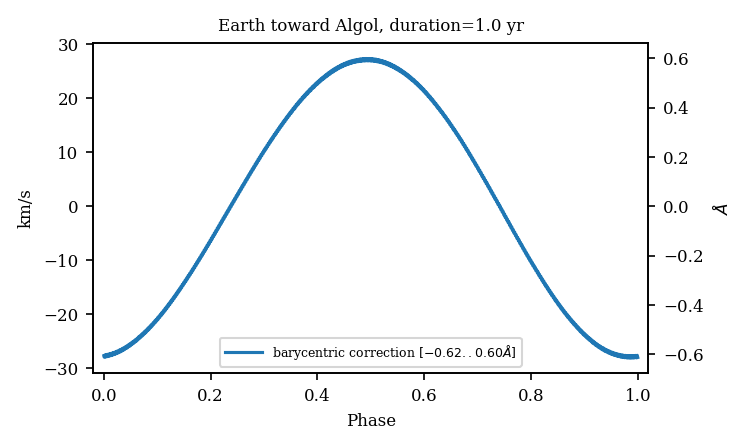
\includegraphics[width=\columnwidth]{img/algol_bary.png}
	\caption{Barycentric correction for the Algol system during a single year}
\end{figure}

Having the stars radial velocity toward earth we can then calculate the redshift:
\begin{equation}
	\label{eq:dl}
	\Delta\lambda_{rv} = \overline{\lambda} \frac{v_{* \rightarrow \earth}}{c}
\end{equation}
with $\overline{\lambda}$ as center wavelength of the observed spectrum and $c$ the speed of light.

It is also possible to derive the redshift from the measured data itself.
One can measure the wavelength difference of absorption line minima between the observed and synthetic spectra.

\paragraph{Modifying spectral resolution}
We also need to apply the resolution of the observed spectrum $RESOL$ to the synthetic spectrum.
We do this by convolution of the synthetic spectrum with a Gaussian kernel having a standard deviation of:
\begin{equation}
	\sigma = 2.543 \frac{\overline{\lambda}}{RESOL}
\end{equation}
$2.543$ is the standard deviation of a Gaussian bell curve with a FWHM\footnote{full width half maximum} of one. See \cite{SablowskiSchanne2018} pp.\ xxx-xxx for an explaination how spectral resolution is defined.

Convolution can be done with the \verb|astropy.convolution.convolve| method applying a \verb|astropy.convolution.Gaussian1DKernel| to the spectrum.

\subsection{Continuum reduction}

\paragraph{Masking}
Before we continue, calculating the "smooth approximation", as explained in chapter 1,
one additional thought:
We may want to exclude some wavelength regions of the observed spectrum when we know in advance that the observed spectrum does differ significantly from the synthetic one.
In our Algol example we wanted to measure emission features in the center of the $H\alpha$ line.

This exclusion can be done by masking that regions.

\paragraph{Continuum approximation}
Having all in place we are able to calculate a smoothed approximation of the continuum:
\begin{equation}
	cont_{approx} = \argmin_{polynomial} \sum_{\lambda} \left( polynomial - \frac{S_{obs}}{S_{synth}} \right)^2
\end{equation}
As approximation we use a polynomial of a given degree.
The polynomial degree depends on the fitted wavelength range and on properties of the spectrograph.
This is demonstrated in figure \ref{four_spectra}.
If unsure one can use the AIC\footnote{Akaike information criterion} \cite{Akaike1974} to choose the degree that best fits the data.
Fitting can be done with the \verb|numpy.polyfit| method.

The normalized spectrum can then be written as:
\begin{equation}
	spec_{norm} = spec_{obs} / cont_{approx}
\end{equation}

Figure \ref*{normalize_howto} shows the entire process.

\begin{figure}[hb]
	\label{four_spectra}
	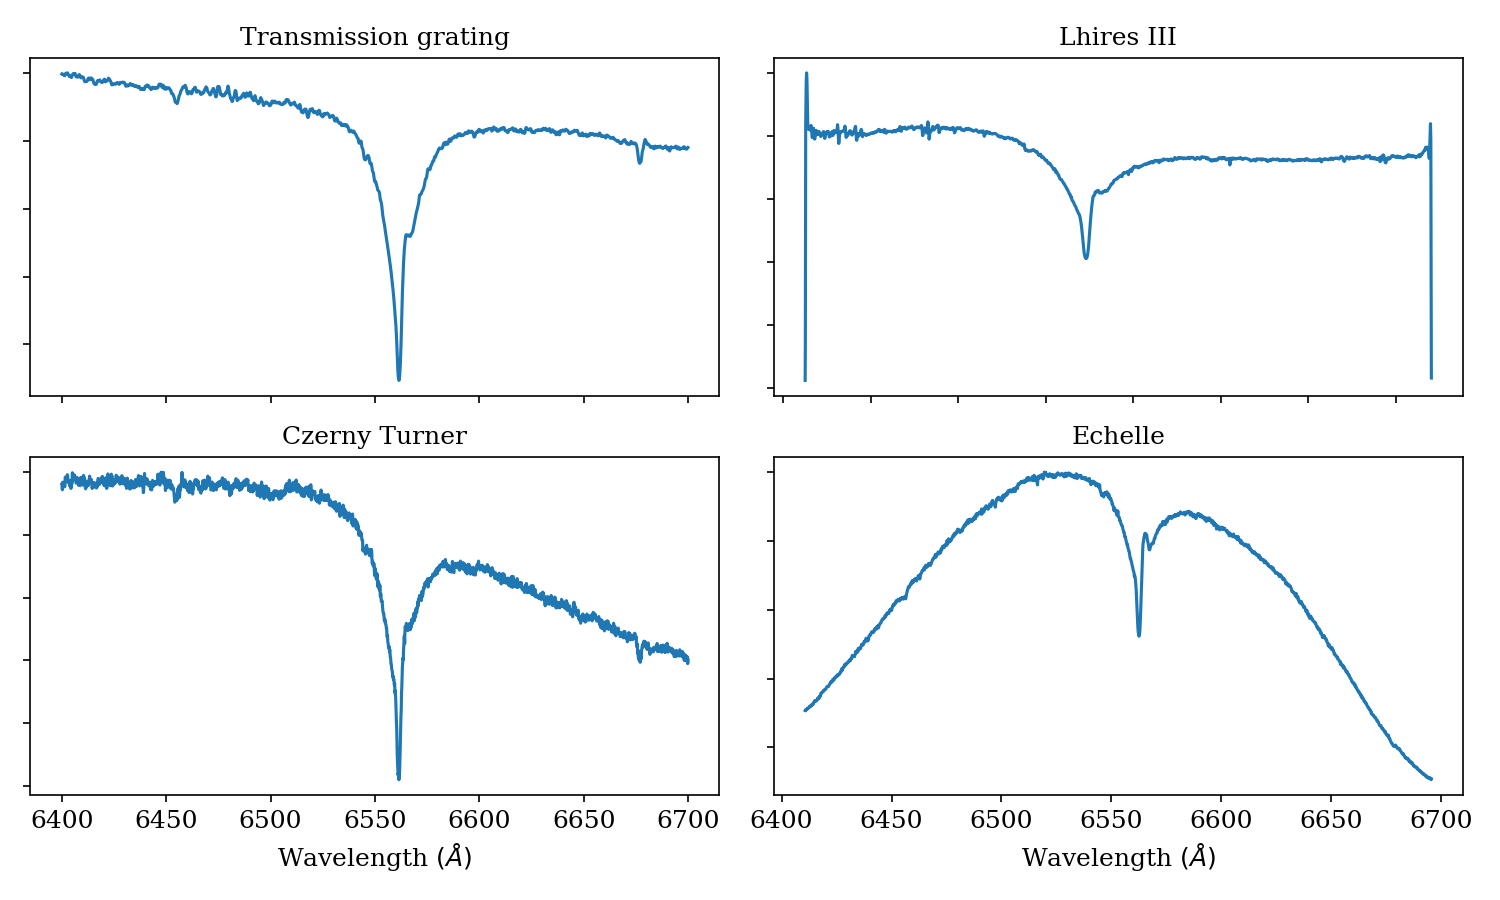
\includegraphics[width=\columnwidth]{img/four_spectra_big.png}
	\caption{$H\alpha$ measured by four different spectrographs. One can see how polynomial of different degree may be required to fit the different spectra.}
\end{figure}

\begin{figure}[hb]
	\label{normalize_howto}
	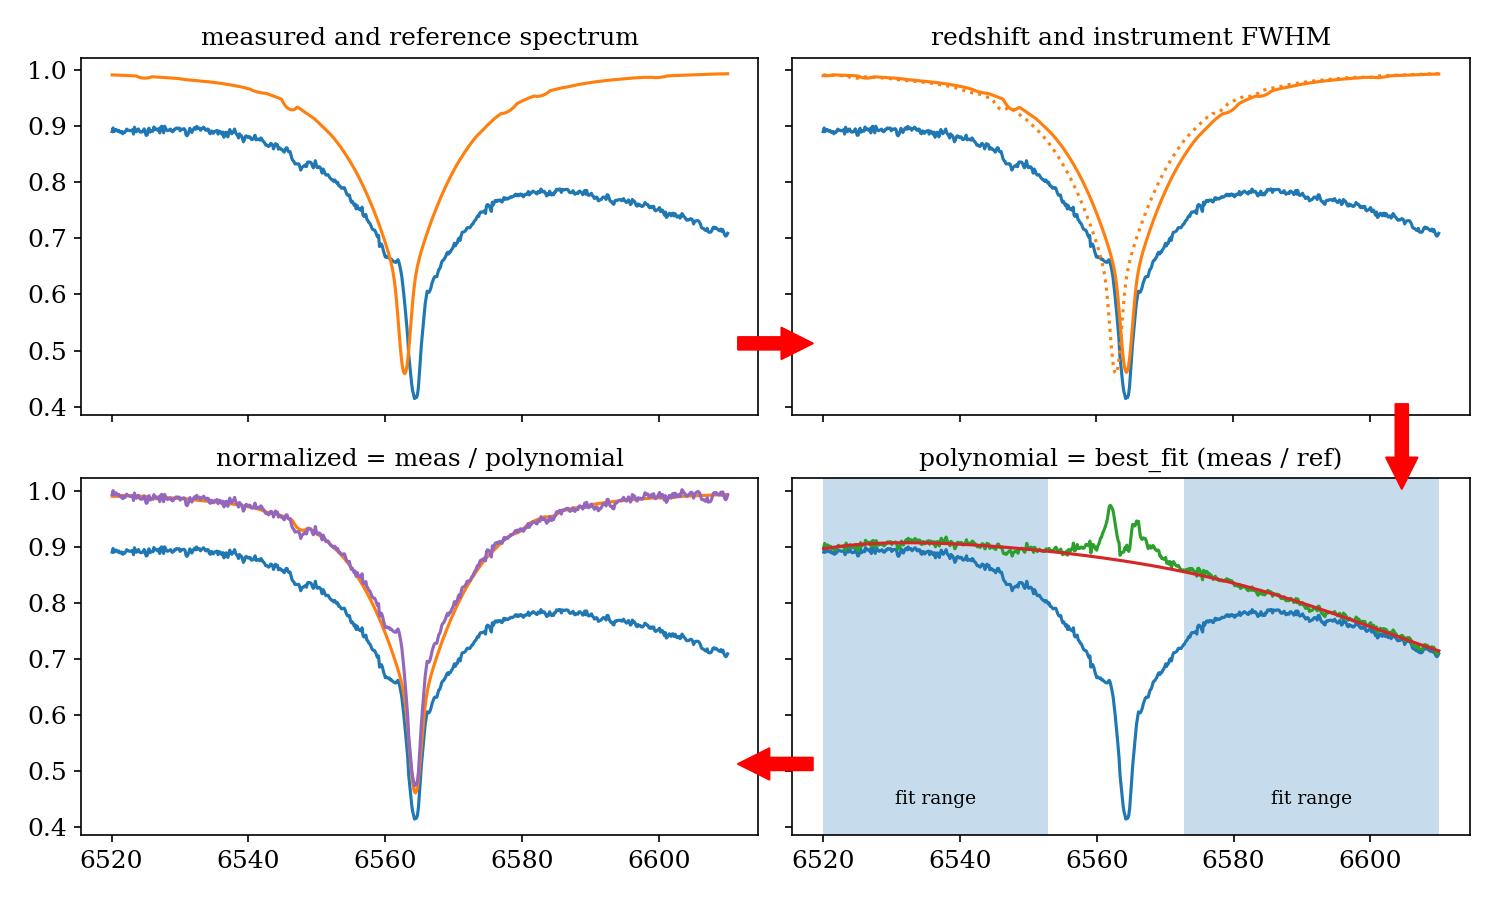
\includegraphics[width=\columnwidth]{img/normalize_howto.png}
	\caption{The entire normalization process containing, redshift, convolution with the FWHM of the instrument resolution, calculation of the best fitting polynomial and finally the normalization. The fit is done in the blue area -- the line center is masked.}
\end{figure}


\section{Conclusions}

\bibliographystyle{apalike}
\bibliography{../../../../Literature/all}

\end{document}
